\documentclass{article}

\usepackage{fancyhdr}
\usepackage{extramarks}
\usepackage{amsmath}
\usepackage{amsthm}
\usepackage{amsfonts}
\usepackage{tikz}
\usepackage[plain]{algorithm}
\usepackage{algpseudocode}
\usepackage{listings}
\usepackage{xcolor}

\usetikzlibrary{automata,positioning}

\definecolor{codegreen}{rgb}{0,0.6,0}
\definecolor{codegray}{rgb}{0.5,0.5,0.5}
\definecolor{codepurple}{rgb}{0.58,0,0.82}
\definecolor{backcolour}{rgb}{0.95,0.95,0.92}

%
% Basic Document Settings
%

\topmargin=-0.45in
\evensidemargin=0in
\oddsidemargin=0in
\textwidth=6.5in
\textheight=9.0in
\headsep=0.25in

\linespread{1.1}

\pagestyle{fancy}
\lhead{Yousef Alaa Awad}
\chead{\hmwkClass\: \hmwkTitle}
\rhead{\firstxmark}
\lfoot{\lastxmark}
\cfoot{\thepage}

\renewcommand\headrulewidth{0.4pt}
\renewcommand\footrulewidth{0.4pt}

\setlength\parindent{0pt}

%
% Create Problem Sections
%

\setcounter{secnumdepth}{0}
\newcounter{partCounter}
\newcounter{homeworkProblemCounter}
\setcounter{homeworkProblemCounter}{1}

\newcommand{\hmwkTitle}{Homework\ \#1}
\newcommand{\hmwkDueDate}{September 8, 2025}
\newcommand{\hmwkClass}{Computer Architecture, Section 379}

%
% Title Page
%

\title{
    \vspace{2in}
    \textmd{\textbf{\hmwkClass:\ \hmwkTitle}}\\
    \normalsize\vspace{0.1in}
    \vspace{3in}
}

\author{Yousef Alaa Awad}

% Problems start here
\begin{document}

\maketitle
\pagebreak

\section{1}
\textbf{Given:} Translate the high-level language code below into assembly instructions. The variables A, B, C, D, E and F are located in the memory and can be accessed by their label (e.g., LOAD R1, A will load A from the memory into R1). Minimize the number of instructions in the assembly code that you write.
$$ F = (A-B)*\frac{(C+D)}{(E-D)} $$

\subsection{A) Write the code for an accumulator architecture}
\begin{centering}
  \begin{displaymath}
  \begin{array}{c | c}
		LOAD\ E  \\
		SUB\ D  & E - D \\
		STORE\ R1 & R1 = E - D\\
		LOAD\ C \\
		ADD\ D  & C + D\\
		DIV\ R1 & \frac{C+D}{R1} = \frac{C+D}{E-D} \\
		STORE\ R1 & R1 = \frac{C+D}{E-D} \\
		LOAD\ A  \\
		SUB\ B  & A - B \\
		MUL\ R1 & (A-B)*\frac{C+D}{E-D} \\
		STORE\ F & End\\
  \end{array}
  \end{displaymath}
\end{centering}
All in all, this takes 11 Instructions and 11 Memory Calls.

\subsection{B) Write the code for a stack architecture. Assume that the division (subtraction) operation divides (subtracts) the topmost value in the stack by the second topmost value.}
\begin{centering}
  \begin{displaymath}
  \begin{array}{c | c}
		PUSH\ D \\
		PUSH\ E \\
		SUB & E-D \\
		PUSH\ C \\
		PUSH\ D \\
		ADD & C+D \\
		DIV & \frac{C+D}{E-D} \\
		PUSH\ B \\
		PUSH\ A \\
		SUB & A-B \\
		MUL & (A-B)*\frac{C+D}{E-D} \\
		POP\ F & End \\
  \end{array}
  \end{displaymath}
\end{centering}
All in all, this takes 12 Instructions and 7 Memory Calls.

\subsection{C) Write the code for a register-memory architecture}
\begin{centering}
  \begin{displaymath}
  \begin{array}{c | c}
		LOAD\ R1,C \\
		ADD\ R1,D \\
		LOAD\ R2,E \\
		SUB\ R2,D \\
		DIV\ R2,R1 & R2= \frac{R1}{R2} = \frac{C+D}{E-D}\\
		LOAD\ R1,A \\
		SUB\ R1,B \\
		MUL\ R1,R2 \\
		STORE\ R1,F & End\\
	\end{array}
  \end{displaymath}
\end{centering}
All in all, this takes 9 Instructions and 7 Memory Calls.

\subsection{D) Write the code for a load-store architecture}
\begin{centering}
  \begin{displaymath}
  \begin{array}{c | c}
		LOAD\ R1,C \\
		LOAD\ R2,D \\
		ADD\ R1,R1,R2 \\
		LOAD\ R3,E \\
		SUB\ R2,R3,R2 & R2=R3-R2=E-D \\
		DIV\ R1,R1,R2 & R1=\frac{R1}{R2}=\frac{C+D}{E-D} \\
		LOAD\ R2,A \\
		LOAD\ R3,B \\
		SUB\ R2,R2,R3 \\
		MUL\ R1,R1,R2 \\
		STORE\ R1,F & End \\
  \end{array}
  \end{displaymath}
\end{centering}
All in all, this takes 11 Instructions and 6 Memory Calls.


\subsection{E) Compare and count the number of instructions and memory accesses between the different ISAs in the previous parts of the questions (a, b, c, and d).}
\begin{centering}
  \begin{displaymath}
  \begin{array}{c | c | c}
		Type & Instructions & Memory\ Calls \\
		Accumulator & 11 & 11 \\
		Stack & 12 & 7 \\
		Register-Memory & \textbf{9} & 7 \\
		Load-Store & 11 & \textbf{6} \\
  \end{array}
  \end{displaymath}
\end{centering}

\newpage

\section{2}
\textbf{Given: } Some architectures support the ‘memory indirect’ addressing mode. Below is an example. In this case, the register R2 contains a pointer to a pointer. Two memory accesses are required to load the data.
$$ \text{ADD}\ R3,@(R2) $$
\subsection{A) The MIPS CPU doesn’t support this addressing mode. Write a MIPS code that’s equivalent to the instruction above. The pointer-to-pointer is in register \$t1. The other data is in register \$t4.}
\begin{centering}
  \begin{displaymath}
  \begin{array}{c | c}
		LOAD\ \$t2,(\$t1) & R1 = R2^* \\
		LOAD\ \$t2,(\$t2) & R1 = R1^* \\
		ADD\ \$r1,\$t4,\$t2 & End \\
  \end{array}
  \end{displaymath}
\end{centering}

\section{3}
\textbf{Given: } Memory Alignment, Big Endian vs. Little Endian: Write C language program to show how your computer stores the 32- bit integer 0x12131415 and the float 34.73. Your program should print byte per line.
\newline
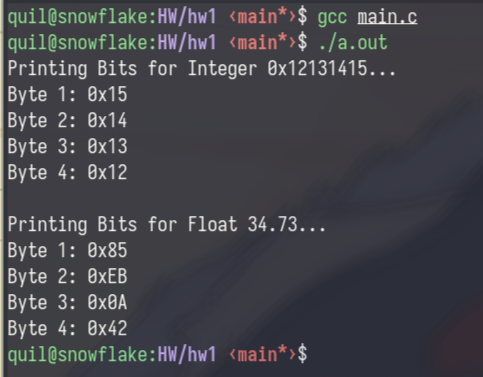
\includegraphics[width=\textwidth]{evidence.png}
\newpage
\lstinputlisting[
	caption=My C Code,
	label={lst:listing-cpp},
	language=C++,
	backgroundcolor=\color{backcolour},   
	commentstyle=\color{codegreen},
	keywordstyle=\color{magenta},
	numberstyle=\tiny\color{codegray},
	stringstyle=\color{codepurple},
	basicstyle=\ttfamily\footnotesize,
	breakatwhitespace=false,         
	breaklines=true,                 
	keepspaces=true,                 
	numbers=left,       
	numbersep=5pt,                  
	showspaces=false,                
	showstringspaces=false,
	showtabs=false,                  
	tabsize=2,
]{main.c}
\newpage

\end{document}
